\documentclass[journal]{IEEEtran}
\usepackage[a5paper, margin=10mm, onecolumn]{geometry}
\usepackage{tfrupee}

\setlength{\headheight}{1cm}
\setlength{\headsep}{0mm}

\usepackage{gvv-book}
\usepackage{gvv}
\usepackage{cite}
\usepackage{amsmath,amssymb,amsfonts,amsthm}
\usepackage{algorithmic}
\usepackage{graphicx}
\usepackage{textcomp}
\usepackage{xcolor}
\usepackage{txfonts}
\usepackage{enumitem}
\usepackage{mathtools}
\usepackage{gensymb}
\usepackage{comment}
\usepackage[breaklinks=true]{hyperref}
\usepackage{tkz-euclide}

\graphicspath{{./figs/}}

\begin{document}
\title{5.3.4}
\author{AI25BTECH11010 - Dhanush Kumar}
\maketitle
\renewcommand{\thefigure}{\theenumi}
\renewcommand{\thetable}{\theenumi}

\textbf{Question}\\
\noindent
Solve the following equations for $x$ and $y$ using cross-multiplication method\\
$
(ax - by) + (a + 4b) = 0 \\
(bx + ay) + (b - 4a) = 0
$\\
\textbf{Solution}\\

The system of equations can be written in vector-matrix form as:
\begin{align}
\myvec{a \\ -b}^T\vec{X} &= -a - 4b \\
\myvec{b \\ a}^T\vec{X} &= 4a - b
\end{align}

Using Cramer's Rule (matrix method), which is algebraically equal to the cross-multiplication method, the solution is obtained as follows.

The coefficient matrix and its determinant are:
\begin{align}
A &= \myvec{a & -b \\ b & a} \\
\det(A) &= a^2 + b^2
\end{align}

The determinant for the first component of $\vec{X}$ is obtained by replacing the first column with the constants:
\begin{align}
A_x &= \myvec{-a-4b & -b \\ 4a - b & a} \\
\det(A_x) &= (-a-4b)a - (-b)(4a-b) \\
&= -a^2 - 4ab + 4ab - b^2 \\
&= -(a^2 + b^2)
\end{align}

The determinant for the second component of $\vec{X}$ is obtained by replacing the second column with the constants:
\begin{align}
A_y &= \myvec{a & -a-4b \\ b & 4a - b} \\
\det(A_y) &= a(4a-b) - b(-a-4b) \\
&= 4a^2 - ab + ab + 4b^2 \\
&= 4(a^2 + b^2)
\end{align}

Finally, using Cramer's Rule, the solution vector is:
\begin{align}
\vec{X} &= \frac{1}{\det(A)} \myvec{\det(A_x) \\ \det(A_y)} \\
\vec{X} &= \myvec{-1 \\ 4}
\end{align}

\begin{figure}[h!]
  \centering
   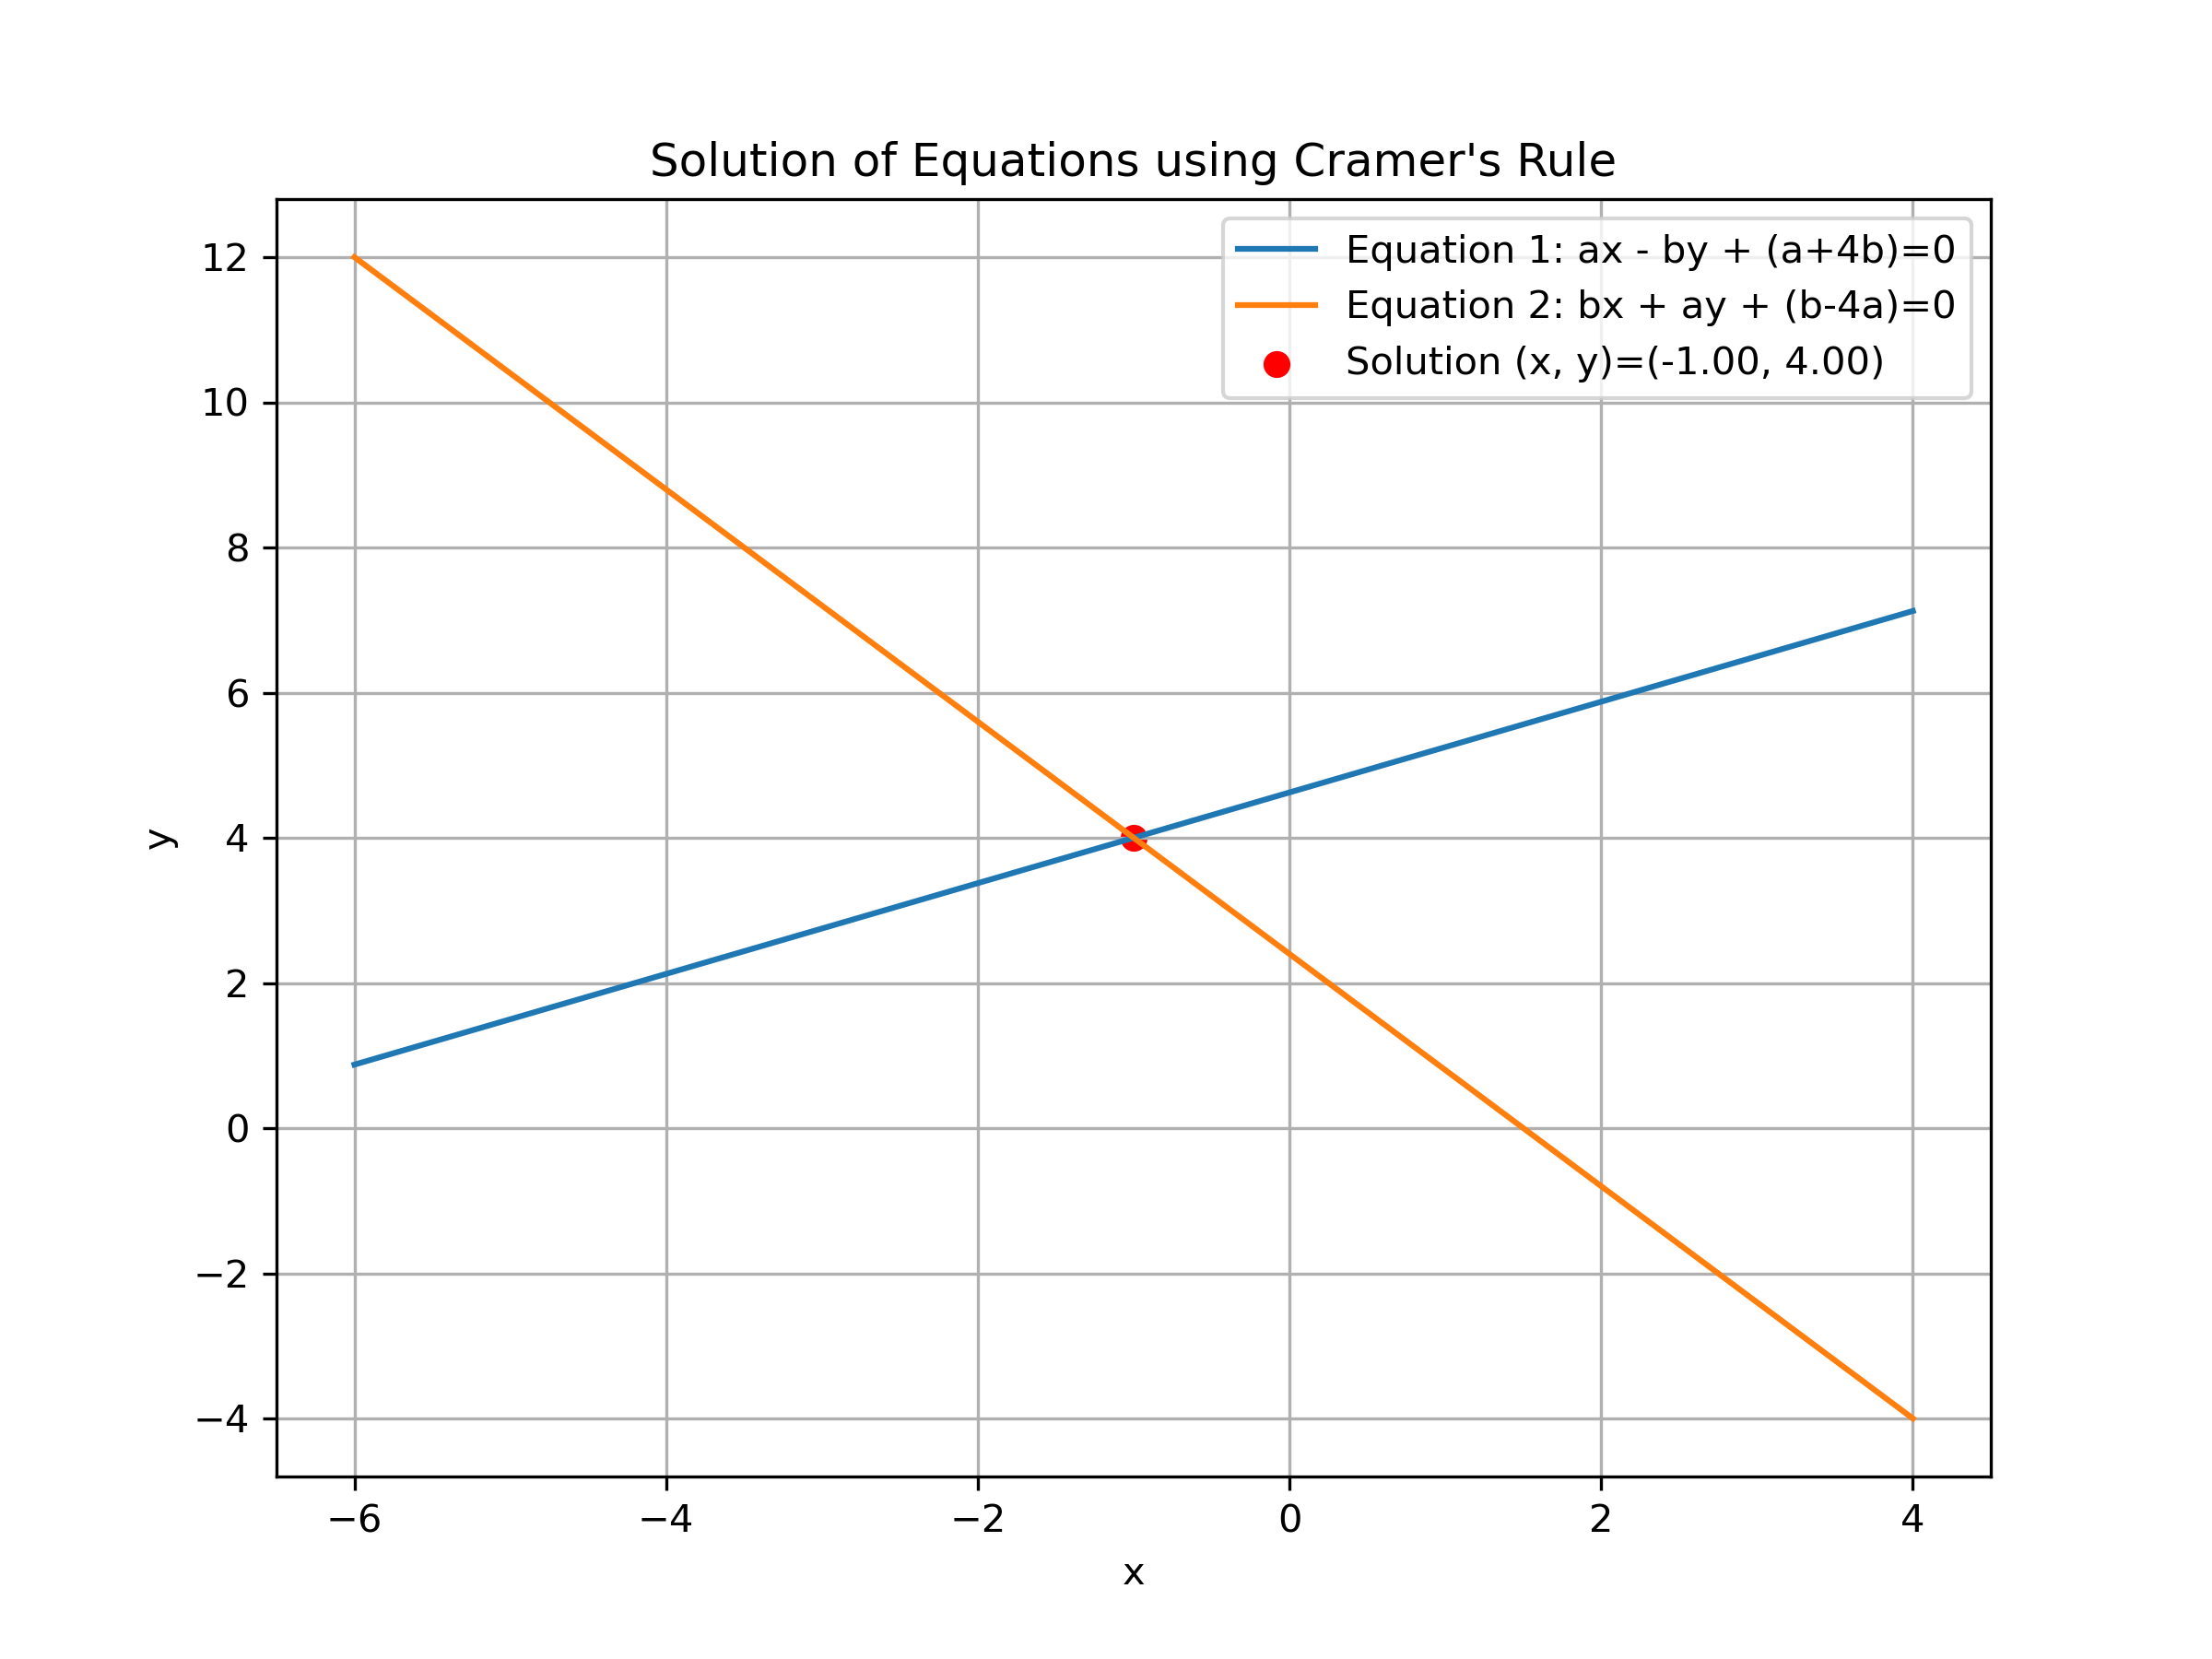
\includegraphics[width=0.7\linewidth]{../figs/equations_solution.png}
   \caption{}
  \label{stemplot}
\end{figure}


\end{document}
